\documentclass[12pt,a4paper]{article}

\usepackage[utf8]{inputenc}
\usepackage[T1]{fontenc}
\usepackage{amsmath,amssymb,amsfonts}
\usepackage{graphicx}
\usepackage{geometry}
\usepackage{bm}
\usepackage{hyperref}
\usepackage{tikz}
\usetikzlibrary{calc,positioning}
\usepackage{pgfplots}
\pgfplotsset{compat=1.18}

\geometry{margin=2.4cm}

\title{\textbf{A Lagrangian Framework for Economic Coherence:\\
Field Dynamics, Phase Alignment, and Emergent Structure}}

\author{Ivan Salines -- Independent Researcher}
\date{November 21, 2025}

\begin{document}
\maketitle

\begin{abstract}
This work introduces a field-theoretic Lagrangian formulation for economic systems composed of multiple interacting subsystems. Each subsystem is described by a density field and a phase field, whose interplay yields coherent structures, stable exchange cycles, and emergent cluster formation. The model is fully dynamical, endogenous, and mathematically grounded, providing a continuum perspective on large-scale economic organization.
\end{abstract}

\section{Introduction}

In conventional economic modeling, aggregate behavior is often described in terms of representative agents, discrete sectors, or reduced dynamical systems that track a small number of macroscopic variables. While such approaches capture important aspects of equilibrium and comparative statics, they typically struggle to represent the emergence of coherent patterns, long-lived organizational structures, and large-scale modes of coordination.

In parallel, field-theoretic methods in physics have proven remarkably effective in describing systems with many degrees of freedom, where macroscopic order arises from local interactions and symmetry principles. Motivated by this analogy, we propose a continuum framework in which an economic system is represented by a set of interacting fields, each associated with a subsystem or sector, and endowed with a density and a phase.

The central object of the theory is a Lagrangian density that encodes local dynamics, interaction structure, and the energetic cost of incoherence. The resulting Euler--Lagrange equations govern the evolution of densities and phases, and naturally give rise to coherent clusters, stable exchange cycles, and emergent macro-structures.

\section{A Field-Theoretic Lagrangian for Economic Interactions}

In this section we introduce a minimal continuum formulation of an economic system composed of multiple interacting subsystems. Each subsystem is characterized by two scalar fields: a \emph{density field} $\rho_i(x,t)$, representing the local concentration of economic resources or productive capacity, and a \emph{phase field} $\theta_i(x,t)$, encoding the orientation of expectations, strategic direction, or collective behavioral alignment.

The goal is not to impose a specific market ideology, but to construct a dynamical framework in which coherent patterns, stable configurations, and large-scale organizational modes emerge naturally from the interplay of density, phase, and interdependence. The resulting structure mirrors the logic of field theories used in physics, while remaining sufficiently general to describe economic phenomena at macro and meso scale.

\subsection{Lagrangian structure}

We postulate that the dynamics of an $N$-component economic system can be captured by the following Lagrangian density:
\begin{equation}
\mathcal{L}
= \sum_{i=1}^{N} \left[
 \rho_i\,\frac{\partial \theta_i}{\partial t}
 - \frac{1}{2}\,\rho_i\,|\nabla \theta_i|^2
 - V_i(\rho_i)
\right]
- \sum_{1 \le i < j \le N}
   J_{ij}\,\rho_i\,\rho_j\,
   \bigl[\,1 - \cos(\theta_i - \theta_j)\,\bigr].
\label{eq:LagrangianGeneral}
\end{equation}

This expression naturally decomposes into two contributions:

\begin{itemize}
    \item A \emph{local component} describing the internal dynamics of each subsystem, governed by its phase evolution, phase gradients, and a local potential $V_i(\rho_i)$ that penalizes over-saturation, scarcity, or structural inefficiencies.

    \item An \emph{interaction component}, weighted by coefficients $J_{ij} \ge 0$, quantifying the strength of interdependence between subsystems $i$ and $j$. The interaction depends on both the densities $\rho_i,\rho_j$ and on their relative phase difference. This structure favors configurations in which strongly connected subsystems tend toward coherent phase alignment.
\end{itemize}

No external drivers are imposed: the model is fully endogenous. Stable configurations arise as those that minimize the effective action associated with~\eqref{eq:LagrangianGeneral}, in complete analogy with variational principles in physics.

\subsection{Interpretation of the terms}

The first term, $\rho_i\,\partial_t \theta_i$, represents the ``kinetic'' contribution associated with time-varying orientations or expectations within subsystem $i$. Changes in direction are more costly when the level of economic activity (as measured by $\rho_i$) is high.

The gradient term $\frac12 \rho_i |\nabla \theta_i|^2$ penalizes spatial incoherence. Large differences in phase over short spatial scales correspond to conflicting strategic orientations within a region or between adjacent sectors, leading to higher energetic cost.

The potential $V_i(\rho_i)$ encodes structural or technological constraints: it stabilizes $\rho_i$ around characteristic values, preventing unbounded accumulation or collapse. In physical terms, $V_i$ acts as a local equation of state for subsystem $i$.

The interaction term,
\[
J_{ij}\,\rho_i \rho_j \bigl[1 - \cos(\theta_i - \theta_j)\bigr],
\]
is central. It assigns an energetic penalty to large phase differences between interdependent subsystems. When $J_{ij}$ is large, even small misalignments between $\theta_i$ and $\theta_j$ can induce significant tension. Conversely, phase coherence between strongly coupled subsystems lowers the interaction energy and contributes to the emergence of large-scale ordered structures.

\subsection{Euler--Lagrange equations}

Applying variational principles to~\eqref{eq:LagrangianGeneral} yields coupled evolution equations for the density and phase fields. Variation with respect to $\theta_i$ gives a continuity-type equation:
\begin{equation}
\frac{\partial \rho_i}{\partial t}
+ \nabla \cdot \left( \rho_i \nabla \theta_i \right)
= \sum_{j \ne i} J_{ij}\,\rho_i \rho_j\,\sin(\theta_i - \theta_j),
\label{eq:rhoEvolution}
\end{equation}
showing that density flows along phase gradients, while relative phase misalignments generate net transfers between subsystems.

Variation with respect to $\rho_i$ leads to a Hamilton--Jacobi-type equation for the phase:
\begin{equation}
\frac{\partial \theta_i}{\partial t}
+ \frac{1}{2} |\nabla \theta_i|^2
+ V_i'(\rho_i)
+ \sum_{j \ne i} J_{ij}\,\rho_j\,
  \bigl[1 - \cos(\theta_i - \theta_j)\bigr]
= 0.
\label{eq:thetaEvolution}
\end{equation}

Together, Eqs.~\eqref{eq:rhoEvolution}--\eqref{eq:thetaEvolution} describe a continuum of interacting subsystems whose large-scale behavior emerges from the interplay of alignment forces, density flows, and structural potentials.

\section{Interpretation and Macroscopic Implications}

The field-theoretic structure introduced above provides a unified lens through which large-scale economic behavior can be analyzed. Although the formulation is fully dynamical and mathematically grounded, several macroscopic implications arise naturally from its geometry.

\subsection{Coherence as an energetic attractor}

The interaction term selects configurations in which subsystems that depend strongly on each other evolve toward phase coherence. This mechanism acts independently of specific institutional arrangements or policy interventions. Coherence is not externally imposed; it is the energetically favorable configuration of the field.

In this sense, coordinated behavior emerges as a low-energy attractor. Fragmented or antagonistic configurations correspond to higher interaction energy and tend to relax toward more coherent states, unless structural asymmetries or external perturbations maintain the system far from equilibrium.

\subsection{Formation of coherence clusters}

In large networks with heterogeneous couplings $J_{ij}$, the system tends to partition into clusters of subsystems whose phases lock together. These ``coherence clusters'' behave as effective macro-entities: within each cluster, resource flows circulate efficiently and tensions are minimized, while between clusters interactions may be weaker or oscillatory.

This phenomenon resembles the formation of solitonic structures in nonlinear field theories, where local coherence extends across a finite region and maintains its identity over long time scales.

\subsection{Resource circulation and efficient exchange cycles}

The continuity equations reveal that phase misalignment drives net transfers of density between subsystems. When phases lock, transfers stabilize into recurrent cycles that conserve global density. Such cycles represent self-organized exchange structures that support long-lived patterns of activity. In this framework, efficient exchange is synonymous with a stable, low-gradient phase configuration.

\subsection{Macroscopic stability}

Global stability corresponds to configurations in which:
\begin{itemize}
    \item phase gradients are small across strongly coupled regions,
    \item internal potentials $V_i$ keep $\rho_i$ within viable operational ranges,
    \item inter-cluster interactions do not produce persistent tension.
\end{itemize}
These conditions define macrostates in which dissipative forces are minimized and structural perturbations propagate smoothly through the network.

\section{Two-Subsystem Dynamics: A Detailed Illustration}

To illustrate the dynamical content of the theory, we analyze the case $N=2$ in a fully uniform spatial configuration. Denoting the two subsystems by $A$ and $B$, the Lagrangian reduces to
\begin{equation}
L = \rho_A \dot{\theta}_A + \rho_B \dot{\theta}_B
    - V_A(\rho_A) - V_B(\rho_B)
    - J\,\rho_A \rho_B \left[1 - \cos(\theta_A - \theta_B)\right].
\end{equation}

The Euler--Lagrange equations yield the coupled system:
\begin{align}
\dot{\rho}_A &= - J \rho_A \rho_B \,\sin(\theta_A - \theta_B), \\
\dot{\rho}_B &= + J \rho_A \rho_B \,\sin(\theta_A - \theta_B), \\
\dot{\theta}_A &= V_A'(\rho_A)
                 + J \rho_B \bigl[1 - \cos(\theta_A - \theta_B)\bigr], \\
\dot{\theta}_B &= V_B'(\rho_B)
                 + J \rho_A \bigl[1 - \cos(\theta_A - \theta_B)\bigr].
\end{align}

\subsection{Conserved quantity}

Summing the density equations,
\[
\dot{\rho}_A + \dot{\rho}_B = 0,
\]
shows that the total density $\rho_{\rm tot} = \rho_A + \rho_B$ is conserved. Thus, no net creation or annihilation of economic value occurs; only redistribution driven by relative phase misalignment.

\subsection{Phase alignment as a stable fixed point}

Defining $\Delta\theta = \theta_A - \theta_B$, the interaction energy takes the form
\[
E_{\rm int} = J \rho_A \rho_B \left[1 - \cos(\Delta\theta)\right].
\]
Its minima occur at $\Delta\theta = 2\pi k, k \in \mathbb{Z}$. Linearizing around these points shows that small deviations satisfy, in a suitable approximation,
\[
\delta\dot{\theta} \approx - J (\rho_A + \rho_B)\, \delta\theta,
\]
indicating exponential relaxation toward phase alignment. Thus, whenever $J > 0$ and both densities are nonzero, the system dynamically selects $\theta_A \approx \theta_B$ as a stable equilibrium.

\subsection{Exchange cycles and oscillatory regimes}

Depending on the shapes of $V_A$ and $V_B$, transient misalignments may produce oscillatory behavior in the phase difference and in the density transfers. These oscillations correspond to recurrent exchange cycles. When damping terms (for example, frictional effects or adjustment costs) are included, the system typically converges toward a stable coherent state.

This minimal example demonstrates how coherent modes arise not from external constraints but from the intrinsic geometry of the interaction term.

\section{Conceptual Figures}

\begin{figure}[h]
\centering
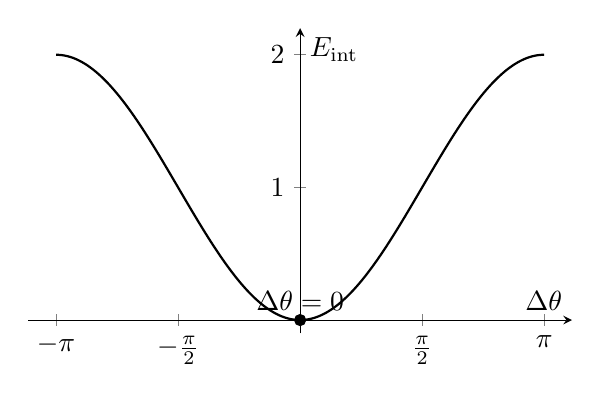
\begin{tikzpicture}
  \begin{axis}[
      width=0.7\textwidth,
      height=0.45\textwidth,
      axis lines=middle,
      xlabel={$\Delta\theta$},
      ylabel={$E_{\mathrm{int}}$},
      xmin=-3.5, xmax=3.5,
      ymin=-0.1, ymax=2.2,
      xtick={-3.1416,-1.5708,0,1.5708,3.1416},
      xticklabels={$-\pi$, $-\frac{\pi}{2}$, $0$, $\frac{\pi}{2}$, $\pi$},
      ytick={0,1,2},
      domain=-3.1416:3.1416,
      samples=200,
      smooth
  ]
    \addplot[thick] {1 - cos(deg(x))};
    \addplot[only marks, mark=*, mark size=2pt] coordinates {(0,0)};
    \node[anchor=south] at (axis cs:0,0) {$\Delta\theta=0$};
  \end{axis}
\end{tikzpicture}

\caption{
Phase alignment diagram for the interaction energy
$E_{\mathrm{int}} \propto 1 - \cos(\Delta\theta)$.
The minimum is attained at $\Delta\theta = 0$, corresponding to coherent evolution.}
\label{fig:phaseAlignment}
\end{figure}

\begin{figure}[h]
\centering
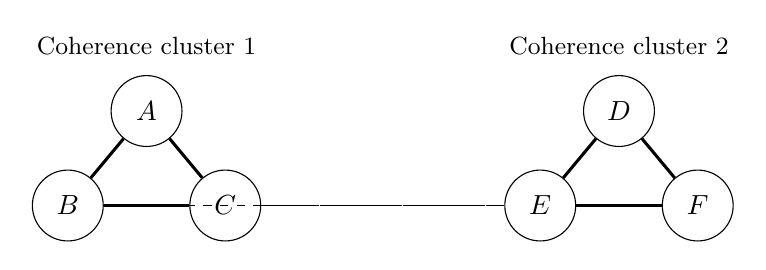
\begin{tikzpicture}[scale=1.0,
    node/.style={circle, draw, minimum size=9mm, inner sep=0pt},
    strong/.style={line width=1.1pt},
    weak/.style={line width=0.6pt, dashed}
]

\node[node] (A) at (-3,  0.9) {$A$};
\node[node] (B) at (-4, -0.3) {$B$};
\node[node] (C) at (-2, -0.3) {$C$};

\draw[strong] (A) -- (B);
\draw[strong] (A) -- (C);
\draw[strong] (B) -- (C);

\node[node] (D) at ( 3,  0.9) {$D$};
\node[node] (E) at ( 2, -0.3) {$E$};
\node[node] (F) at ( 4, -0.3) {$F$};

\draw[strong] (D) -- (E);
\draw[strong] (D) -- (F);
\draw[strong] (E) -- (F);

\draw[weak] (C) -- (E);
\draw[weak] (B) -- (E);

\node[above=4pt of A] {\small Coherence cluster 1};
\node[above=4pt of D] {\small Coherence cluster 2};

\end{tikzpicture}

\caption{
Example of a many-subsystem network with heterogeneous couplings $J_{ij}$.
Strongly connected subsystems form coherence clusters whose phases evolve in unison.
Weak links between clusters allow for interaction without destabilizing internal structure.}
\label{fig:clusters}
\end{figure}

\section{Conclusions}

We have proposed a Lagrangian framework for economic systems in which each subsystem is described by a density field and a phase field, and where interactions are encoded in phase-dependent couplings. The resulting equations of motion naturally generate coherence clusters, stable exchange cycles, and large-scale organizational structures.

This approach suggests several directions for future work, including the calibration of potentials $V_i(\rho_i)$ to empirical data, the exploration of stochastic extensions, and the study of phase transitions between distinct macrostates of economic organization. More broadly, the field-theoretic perspective provides a bridge between the mathematics of organized motion and the phenomenology of complex economic systems.

\end{document}
